
%% LaTeX Beamer presentation template (requires beamer package)
%% see http://bitbucket.org/rivanvx/beamer/wiki/Home
%% idea contributed by H. Turgut Uyar
%% template based on a template by Till Tantau
%% this template is still evolving - it might differ in future releases!

% \documentclass[draft]{beamer}
% \documentclass[handout]{beamer}
\documentclass{beamer}
% \usepackage{pgfpages} %for two screen presentations
% \pgfpagesuselayout{2 on 1}[a4paper,border shrink=5mm] %for handout!
% \setbeameroption{show notes} 
% \setbeameroption{show notes on second screen}
% \setbeameroption{show next slide on second screen}
% \setbeameroption{second mode text on second screen=left}
\setbeamertemplate{navigation symbols}{}

\mode<presentation> 
{
\usetheme{Warsaw} 
% \usetheme{Frankfurt}
% \usetheme{Berkeley}
\usecolortheme{seahorse}
% \usecolortheme{rose}
\usefonttheme[onlylarge]{structuresmallcapsserif}
\usefonttheme[onlysmall]{structurebold}

\setbeamercovered{transparent}
\setbeamercolor{title}{fg=blue!90!black,bg=red!70!white}
}

\usepackage[english]{babel}
\usepackage[latin1]{inputenc}

% font definitions, try \usepackage{ae} instead of the following
% three lines if you don't like this look
\usepackage{mathptmx}
\usepackage[scaled=.90]{helvet}
\usepackage{courier}

\usepackage[T1]{fontenc}

\usepackage{amsmath}
\usepackage{amscd}
\usepackage{amssymb}
\usepackage{amsfonts}
\usepackage{amsthm}
\usepackage{amsfonts}
\usepackage{amsthm}

\usepackage{tikz}
\usepackage{subcaption}
\usepackage{subfigure}

\usepackage{aviolov_style}
\usepackage{local_style}


\title[Spike-Control for Neurons]{Optimal Control of First-Passage Times
in an Ornstein-Uhlenbeck Model
}
% - Use the \inst{?} command only if the authors have different
%   affiliation.
\author{Alexandre Iolov}
% \institute{Annual Meeting in the Statistics Network, Holte}
\date{August 20, 2013}
% % This is only inserted into the PDF information catalog. Can be left
% % out.
% \subject{Talks}

% If you have a file called "university-logo-filename.xxx", where xxx
% is a graphic format that can be processed by latex or pdflatex,
% resp., then you can add a logo as follows:
% \pgfdeclareimage[height=0.5cm]{university-logo}{university-logo-filename}
% \logo{\pgfuseimage{university-logo}}
% Delete this, if you do not want the table of contents to pop up at
% the beginning of each subsection:
% \AtBeginSubsection[]
% {
% \begin{frame}<beamer>
% \frametitle{Outline}
% \tableofcontents[currentsection,currentsubsection]
% \end{frame}
% }

% If you wish to uncover everything in a step-wise fashion, uncomment
% the following command:
%\beamerdefaultoverlayspecification{<+->}

\begin{document}

\begin{frame}
\titlepage
\end{frame}

% \section*{Outline}
\begin{frame}
\tableofcontents[pausesections]
\end{frame}

\section{Problem Background}
\subsection[LIFs]{Leaky Integrate-and-Fire Basics}
\begin{frame}
\frametitle{The Underlying Model}
% \framesubtitle{Subtitles are optional}
A voltage, $X_t$ autonomously decays to zero, is driven and spikes when it hits
threshold:
\begin{columns}[T]
\begin{column}{5cm}
\begin{equation*}
\begin{gathered}
dX_t = (\m + \a(t) - \frac{X_t}{\tc} ) \intd{t} + \b \intd{W_t},
\\
X(0) = .0,
\\
X(\ts) = \xth \implies
\begin{cases}
\ts \sim \text{spike time} 
\\
X(\ts^+) = .0 &
\end{cases}
\end{gathered}
\end{equation*}
\end{column}
\begin{column}{5cm} 
\onslide<2->{
  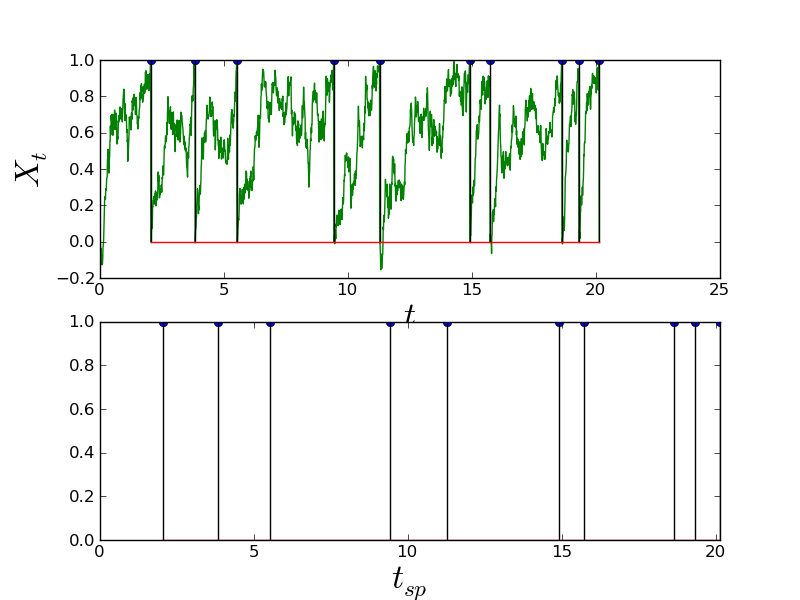
\includegraphics[width=.99\textwidth]{Figs/sinusoidal_train_N=10_example.png}
}
\end{column}
\end{columns}

\pause
\begin{center}
$\a(.) \sim$ the control

$\a(t)\in [\amin,\amax]$
\end{center}

%\usepackage{graphics} is needed for \includegraphics
% \begin{figure}[htp]
% \begin{center}
%   \caption[labelInTOC]{Example Voltage Trajectory + Spikes}
%   \label{fig:voltage_spikes_example}
% \end{center}
% \end{figure}

% \note[item]{When $X$ hits $\vt$, we have a spike}
% \note[item]{$\a$ is our control and is completely determined by us}
\end{frame}

\subsection{Problem Objective}
\begin{frame}
\frametitle{Our Goal}
\only<1-2>{
Impose a pre-specified spike sequence,  $\{t_n\}_1^N$, on the neuron.

\begin{figure}
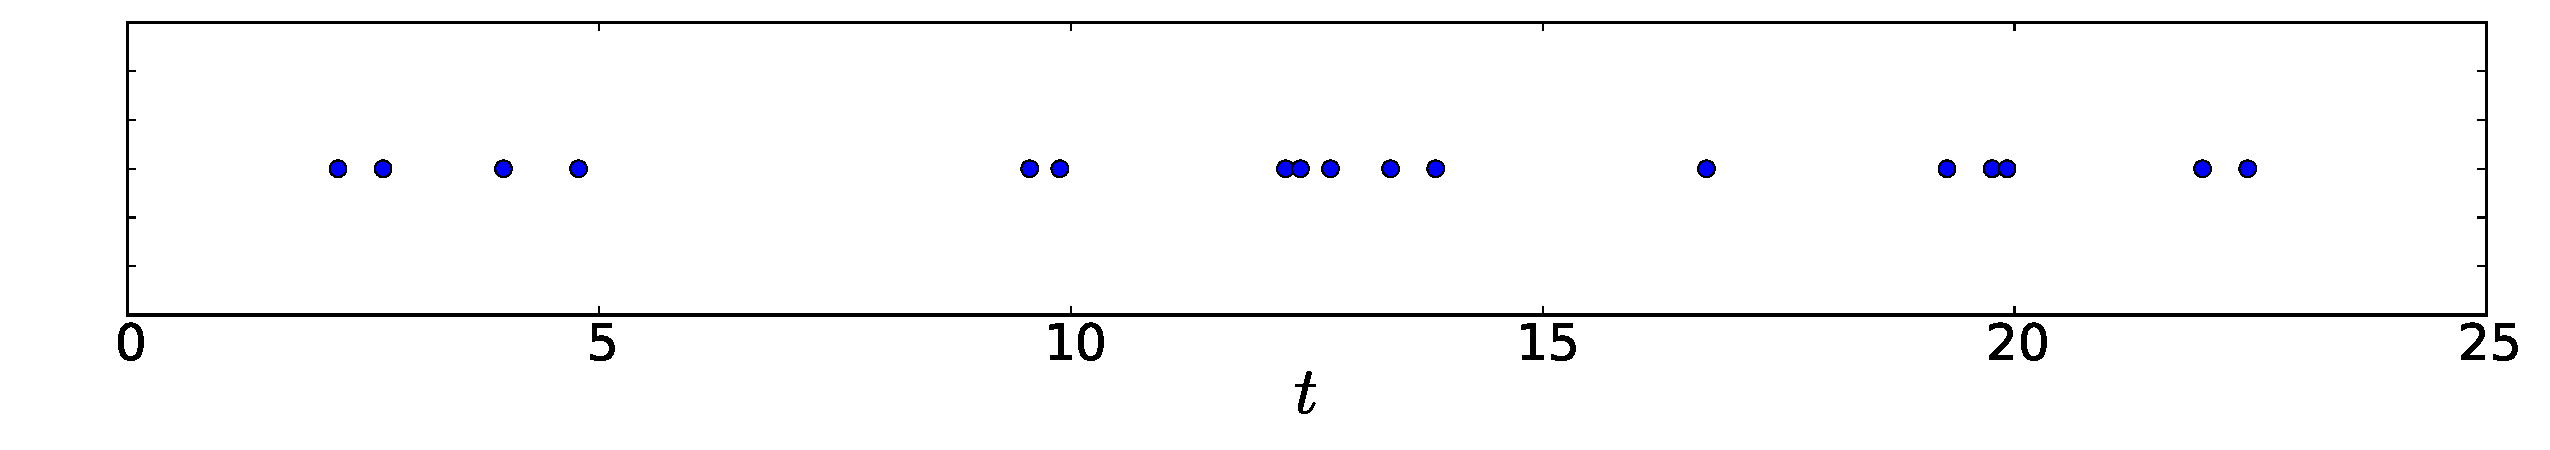
\includegraphics[width=0.9\textwidth]
{Figs/TrainController/target_train_Ahmadian.pdf}
\end{figure}
}
\onslide<2>{
\vskip 3pt

ASSUMPTION: We know when actual spikes, $\{t_{sp,n}\}$ occur
$\implies$ we can work sequentially:

$$
\T = t_n - t_{sp, n-1}
$$

\vskip 3pt

i.e. {\sl Greedy} approach: optimize each interval independently.
}
\end{frame}

\begin{frame}
\frametitle{Our Goal}

Given a target $\T$ find $\a(t)$ minimizing $\Exp[(\T - \ts)^2]$

\vskip2pt 
\\
\begin{figure}  
\begin{center}
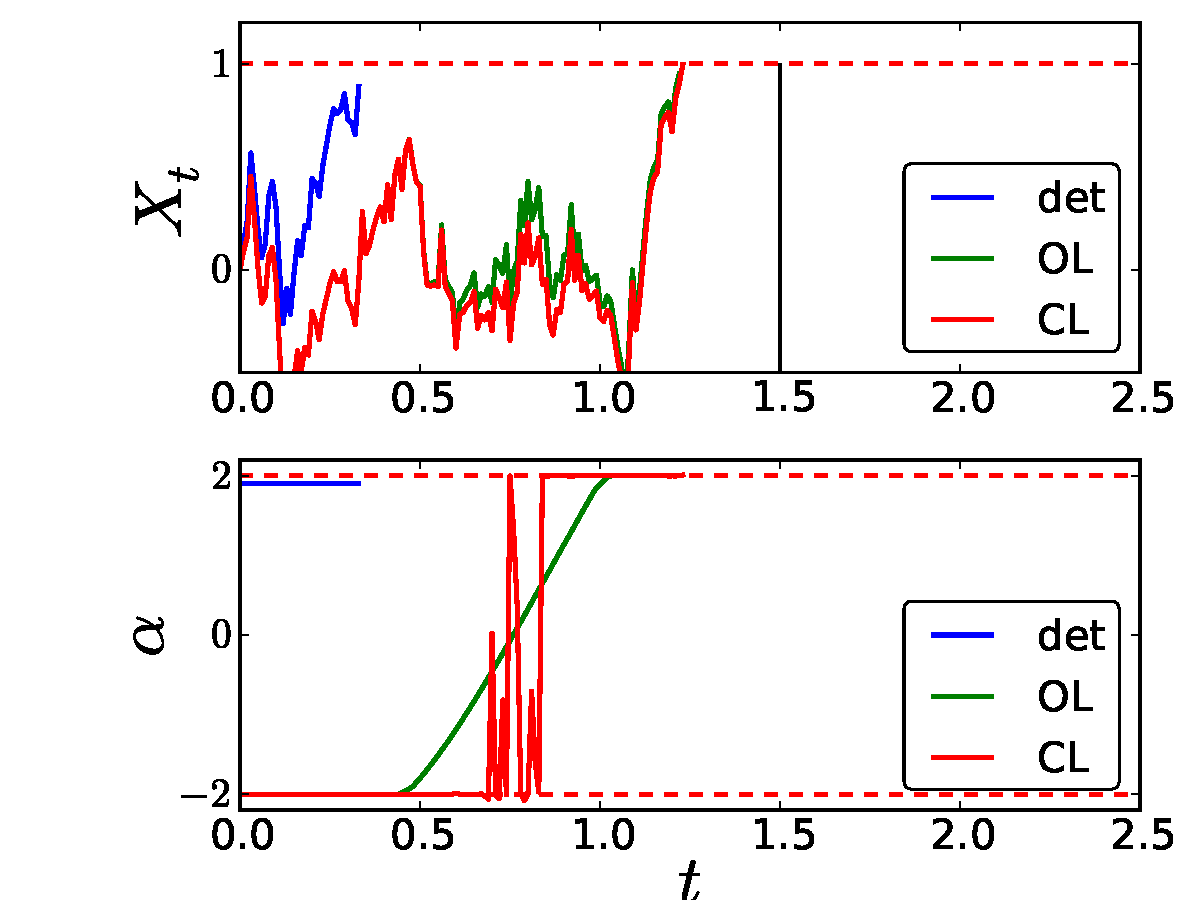
\includegraphics[width=0.9\textwidth,height=.6\textheight]
{Figs/ControlSimulator/SubTHighNoise_pres_Traj2.pdf}
\caption{ Controlled Trajectory Example
- observed vs.\ desired spike time 
}
\end{center} 
\end{figure}

\end{frame} 


\begin{frame}
% \frametitle{Formal Problem Statement}

\begin{block}{Formal Problem Statement}
Given, $\m, \tc, \b$, $\T$ and $X_0 = .0$, find

\begin{equation}
\a(t) = \argmin_{\a(t)} \Big\{ \, J[\a] = 
\Exp\left[
(\ts - \T \big)^2 
+  
\e \int_0^\ts  \a^2(t) \intd{t}  \right]
\, \Big\}
\end{equation}
\end{block}
\end{frame}

\begin{frame}
\frametitle{Control Horizon}
Since we know if and when a spike occurs
$$
t>\T \implies \a(t) = \amax
$$ 
So our control problem takes place over the interval
$$  t \in [0 , \T] $$ 
\end{frame}

 
\section{Closed-loop stochastic control - dynamic programing}
\begin{frame}
\frametitle{Dynamic Programing Solution}
If we have state observations / feedback
\vskip2pt
$\implies$ Dynamic Programming /
Hamilton-Jacobi-Bellman (HJB) Equations
\vskip 1pt
\only<2>{
\begin{equation*}
\begin{gathered}
\di_t \underbrace{v(x,t)}_{\textrm{value function}} + \tfrac{\b^2}{2} \di_x^2 v
+ \e \a^2 + (\a -\tfrac{x}{\tc}) \di_x v 
= 0
\\
\begin{cases}
v(\xth,t) = (s-\T)^2  \quad & \textrm{BC}
\\
% \di_x v(\xmin, t)  = .0  \quad &\textrm{lower BC}
% \\
v(x,\T)  = \Exp[ (\t^2 : X_{\T+\t} = \xth) \,|\,X_\T = x, \a(t) = \amax]  \quad&
\textrm{TC}
\end{cases}
\\
\a (x,t) = \min \left(\amax,
		 \max\left(\amin, -\frac{\di_x v(x,t)}{2\e}\right)
\right)
\end{gathered}
\label{eq:OC_LS_HJB_full}
\end{equation*}
}
\only<3>{
%\usepackage{graphics} is needed for \includegraphics
\begin{figure}[htp]
\begin{center}
  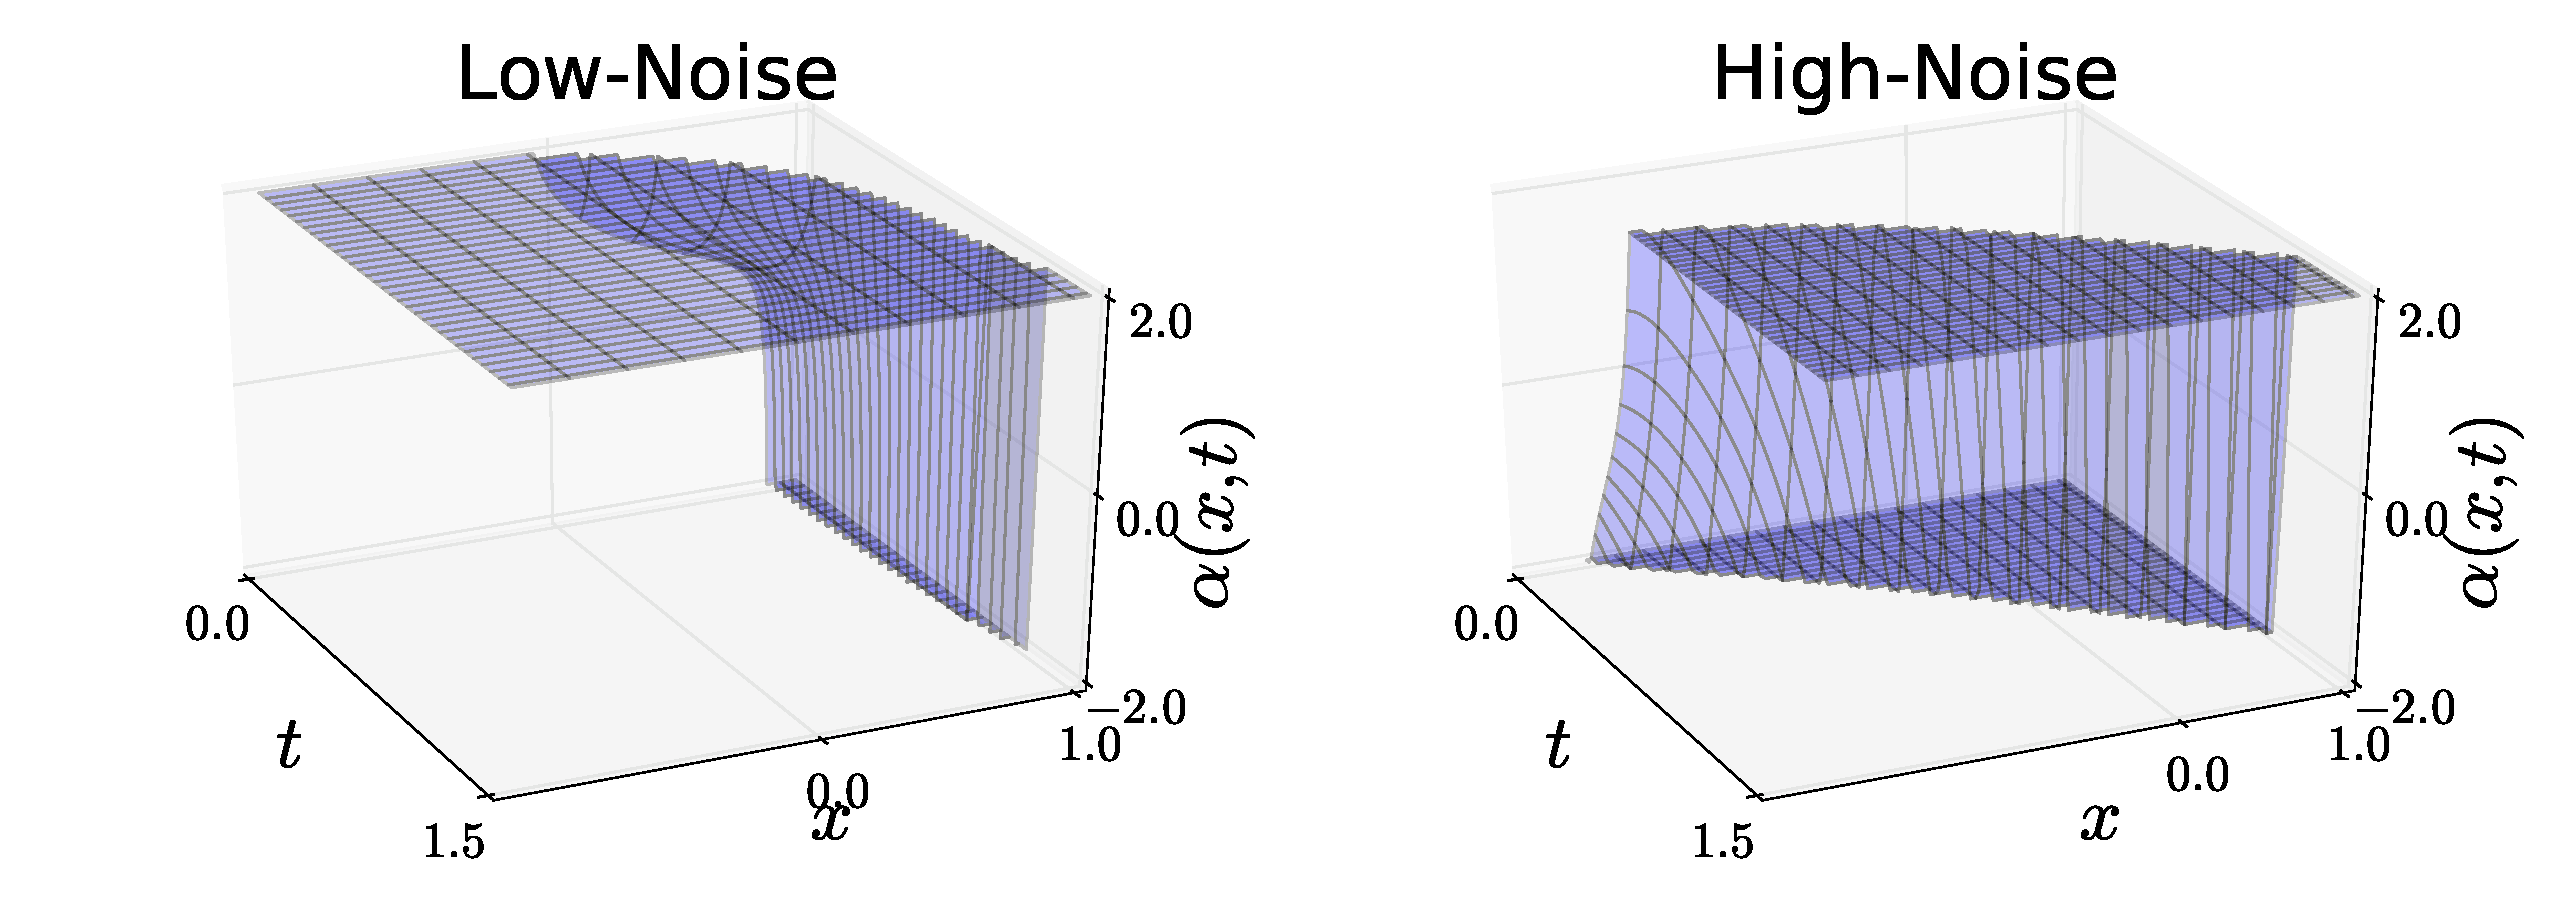
\includegraphics[width=.9\textwidth]
  {Figs/HJB/Regimes_presentation_control_surf.pdf}
  \caption[]{Closed-Loop Control Solution}
\end{center} 
\end{figure}
}
\end{frame} 


% \begin{frame}
% Simplest solution $\sim$ ignore the noise!
% 
% $\implies$ Deterministic Optimal Control (in 1-D)
% 
% 
% \begin{figure}
% \begin{center}
%   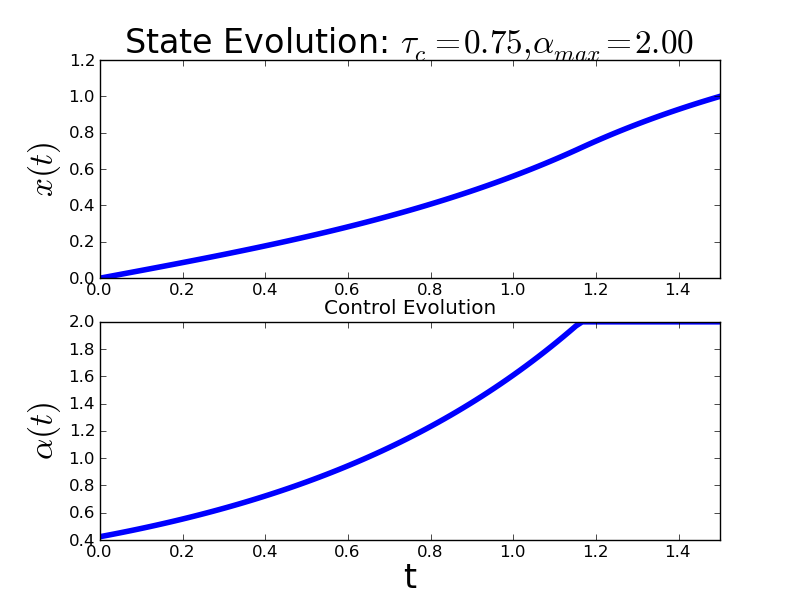
\includegraphics[width=.6\textwidth]{Figs/ControlSimulator/deterministic_example.png}
%   \caption{An example trajectory for the deterministic dynamics. }
% \end{center}
% \end{figure}
% 
% \end{frame}
% 
% \begin{frame}
% \frametitle{An Unfair Comparison}
% 
% \only<1>{
% \begin{figure}[b]
% \begin{center}
% \subfloat
% {
% \includegraphics[width=0.4\textwidth]
% {Figs/ControlSimulator/example_controlled_trajectories_id4.png}
% }
% \subfloat
% {
% \includegraphics[width=0.4\textwidth]
% {Figs/ControlSimulator/example_controlled_trajectories_id3.png}
% }
% \caption[]{Controlled trajectories using deterministic
% vs. stochastic control approaches. $\T$ is indicated with the red vertical
% line, $\tc, \b = [.75, 1.25]$.}
% \end{center}
% \end{figure}
% \note[item]{In A the performance of both
% control laws is essentially the same, but in B we see the advantage of the
% stochastic approach}
% }
% \only<2-3>{
% \begin{table}[b]
% \centering
% \begin{tabular}{lcc}
% Control Law & Empirical Error & Theoretical Error
% \\
% \hline
% Open-Loop Deterministic &  0.647  \onslide<3>{$\swarrow$} &  - \\
% Closed-Loop  Stochastic &  0.336  \onslide<3>{$\nwarrow$} &  0.285 \\
% \end{tabular}
% \caption{Realized performance of the different control laws. The Error is $\Exp
% \left[ (\T - \ts)^2 \right] $}
% \label{tab:realized_avg_errors_det_vs_stoch}
% \end{table}
% }
% \onslide<3>{
% \vskip 5pt
% \begin{center}
% Can we do better?
% \end{center}
% }
% \end{frame}


\section{Open-loop Stochastic Control - maximum principle}

\begin{frame}
\frametitle{Maximum Principle Solution}
If we do NOT have state observations / feedback
\vskip2pt
$\implies$ Maximum Principle /
 Forward-Backward Kolmogorov Equations
\only<2>{ 
\begin{equation*}
\begin{gathered}
\begin{aligned}
\di_t \overbrace{f(x,t)}^{\textrm{density}} =
				\frac{\b^2 }{2}\cdot \di^2_x f -
 				\di_x \Big[ \left( \m + \a(t)- \frac{x}{\tc}\right)  \cdot f \Big]
\\
\\
\frac{\b^2}{2}\cdot \di^2_x p +
			(\m + \a(t)- \frac{x}{\tc})  \cdot \di_x p  
 =& -\di_t \underbrace{p(x,t)}_{\textrm{adjoint}}
\end{aligned}
\\
\begin{cases}
	 f(x,0) &=  \delta(x)  
	\\
	f(\xth,t) &=  0
\end{cases} \, 
\vline\,
\left.
\begin{array}{rcl}
	\Exp[ (\t^2 : X_{\T+\t} = \xth) \,|\,X_\T = x,\amax]  
	&=&  
	p(x,\T) 
	\\
	 (s-T)^2
	&=&
	p(\xth,t) 
\end{array}\right\}  
\\
\a (t) = \min \left(\amax,
		 \max\left(\amin, -\frac{\smallint p(x,t) \cdot \di_x f(x,t)
		 \intd{x}}{2\e}\right)\right)
\end{gathered}
\end{equation*}
}
\only<3>{
%\usepackage{graphics} is needed for \includegraphics
\begin{figure}[htp]
\begin{center}
  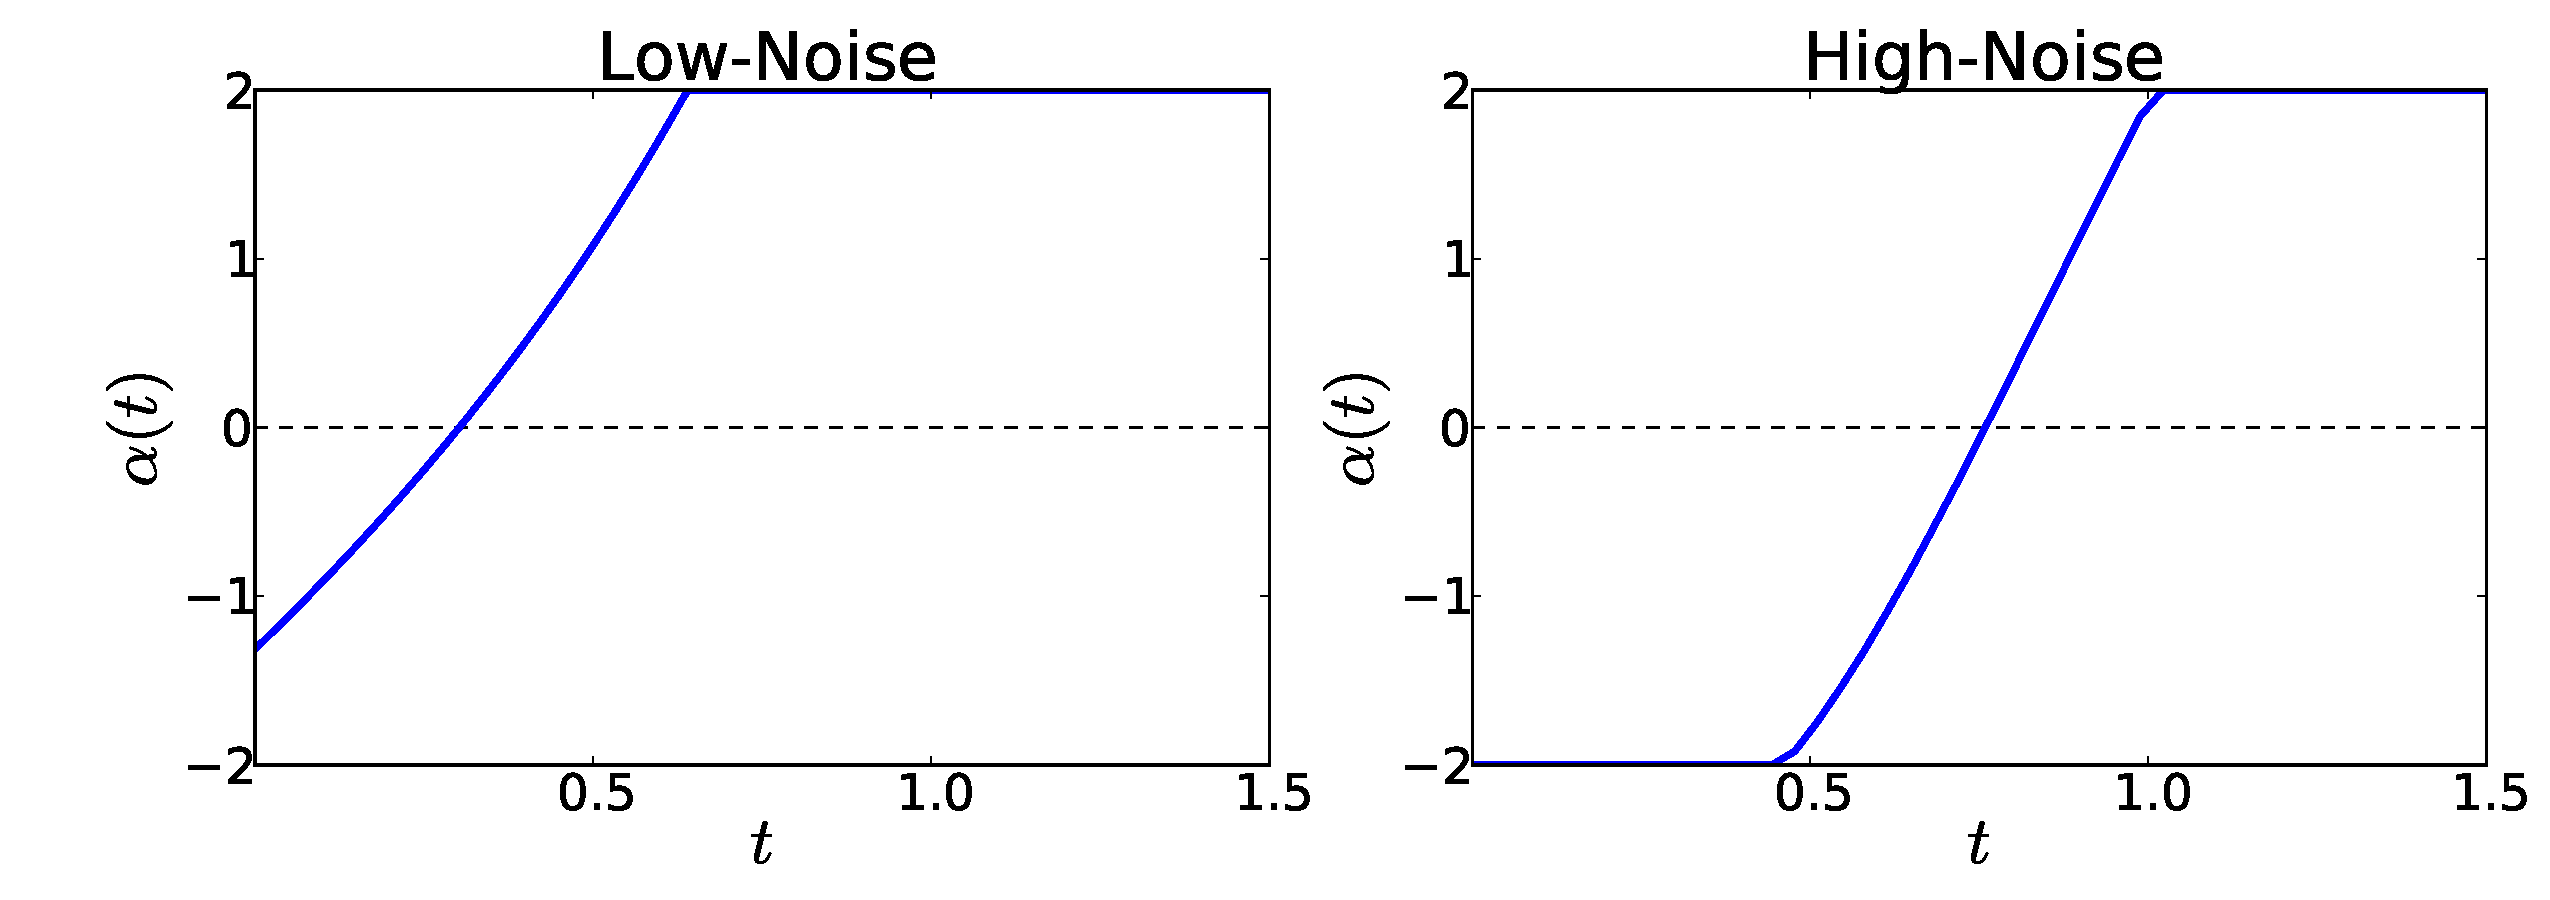
\includegraphics[width=.95\textwidth]
  {Figs/FP_Adjoint/SubT_Regimes_cs_presentation.pdf}
  \caption[labelInTOC]{Open-Loop Control Solution} 
\end{center}
\end{figure} 
%\vfill
}
\end{frame} 

% \begin{frame}
% \frametitle{Maximum Principle Solution}
% Consider, $f(x,t)$, the forward transition density for $X_t$
% \vskip 2pt
% \only<1>{
% \vskip 10pt
% \begin{align*}
% \Exp\left[
% (\ts - \T \big)^2 \right]
% =&
% \int_0^\ts (t-\T)^2 \cdot \left( - \frac {\b^2} 2 \di_x f(\xth, t) \right) 
% \intd{t}
% \\
% &+
% \int_\xmin^\xth 
% \Exp[\t^2|x, \amax] \cdot f(x,\T) \intd{x}
% \end{align*}
% \vskip 12pt
% }
% \only<2-3>{
% \begin{center}
% \begin{tikzpicture}[scale = 1.5]
% \draw[->][dashed] (-.75, 1.) --
% 		node[at start, left]{$\xth$}
% 		node[at end, right] {$t$}
% 		(1.9,1.);
% 		
% \draw[->][very thick] (.1, .5) --
% 		node[at start, left] 
% 			{$\Big[(t-\T)^2 \cdot \tfrac{-\b^2} 2 \di_x f\Big]$}
% 		node[at end , above]{``EARLY''}
% 		(.5,1.25);	
% 
%  \draw[->][dashed] 		
% 		(1.5,-.0) --
% 		node[at start, below]{$\T$}
% 		node[at end, above]{$x$}
% 		(1.5,1.25) ;
% 		
% 		\draw[->][very thick] (1.2, .0) --
% 		node[at start, left] {$\Big[\Exp[\t^2|x, \amax] \cdot f\Big]$}
% 		node[at end , right]{``LATE''}
% 		(1.8,.5);	 
% \end{tikzpicture}
% \end{center}
% }
% \vskip 1pt
% \indent $f(x,t) \sim$ deterministic (it satisfies a Fokker-Planck equation)
% \begin{align*}
% \di_t f(x,t) =& -\di_x \left[(\a(t) - \frac{x}{\tc} )  f \right] + 
% \frac{1}{2}\di^2_x \left[\b^2 f \right]
% \end{align*}
% 
% \vskip 2pt
% $\implies$ optimize using $f$
% \vskip 2pt
% 
% \onslide<3>{
% \begin{center}
% But how do we optimize with PDEs?
% \end{center}
% }
% \end{frame}
% 
% \begin{frame}
% \frametitle{Lagrange Multipliers for PDEs}
% \begin{align*}
% J[\a]
% =&
% \int_\xmin^\xth 
% \underbrace{\Exp[\t^2|x, \amax]}_{\Ttwo(x)} \cdot f(x,\T) \intd{x}
% \\
% &+ \int_0^\ts (t-\T)^2 \cdot \left( - \frac {\b^2} 2 \di_x f(\xth, t) \right) 
% \intd{t}
% \end{align*}
% \\
% \pause
% \begin{align*}
% &+ \int_0^\ts\int_\xmin^\xth
% \underbrace{p(x,t)}_{\textrm{co-state}} \cdot \underbrace{(\di_t f -
% (-\di_x \big[(\a(t) - \frac{x}{\tc} )  f \big] + \frac{1}{2}\di^2_x \left[\b^2 f \right] ))}_{\textrm{F-P eq'n}}
% \intd{x}\intd{t}
% \end{align*}
% \pause
% Optimality Principle:
% $$
% \frac{\delta J}{\delta \a} = 0 
% $$
% \end{frame}
% 
% % \begin{frame}
% % \frametitle{Forward-Backward System}
% % \begin{minipage}{0.48\linewidth}
% % \begin{tikzpicture}[scale = .8]
% % \draw[->] (-.25,1) -- node[above]   {$f$} node[below]{State}
% % 	(4.5,1) ;
% % \end{tikzpicture}
% % 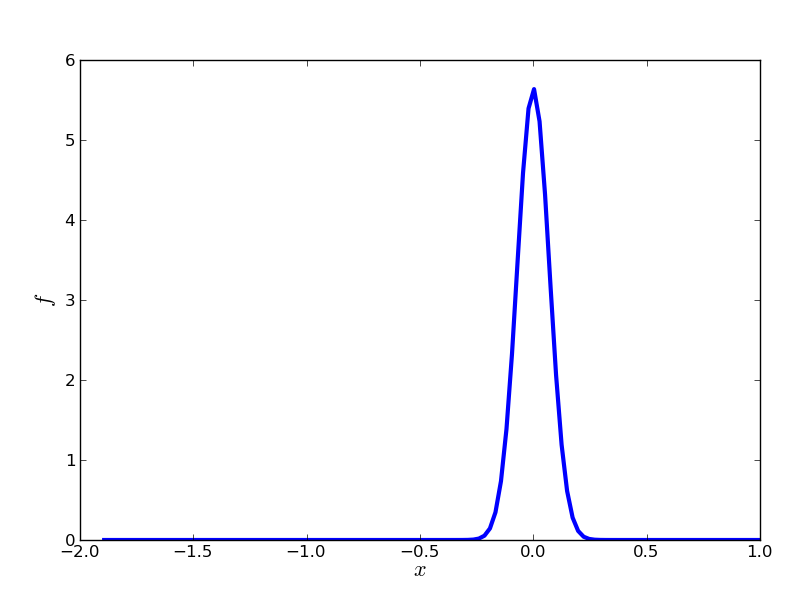
\includegraphics[width=0.75\textwidth]{Figs/FP_Adjoint/Stylized__f.png}
% % \end{minipage}
% % \vline 
% % \begin{minipage}{0.48\linewidth}
% % \begin{flushright}
% % 
% % 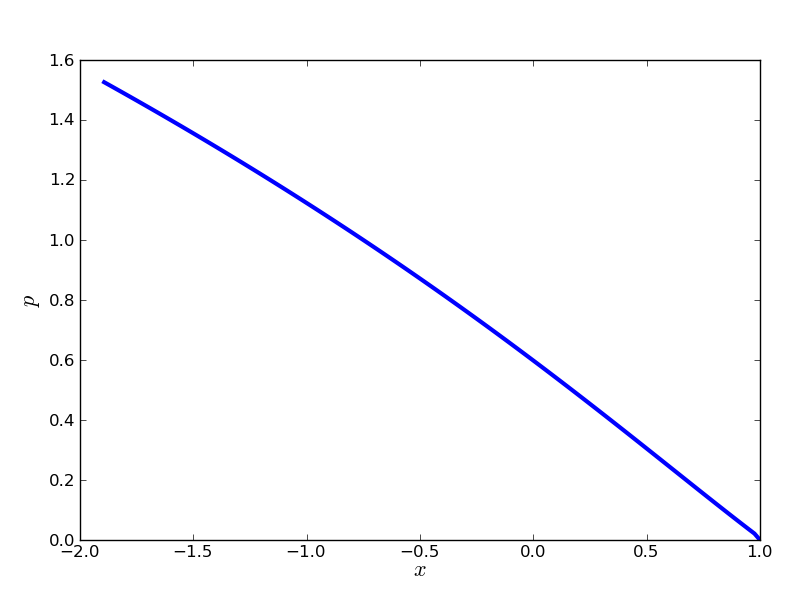
\includegraphics[width=0.75\textwidth]{Figs/FP_Adjoint/Stylized__p.png}
% % 
% % \begin{tikzpicture}[scale =.8]
% % \draw[<-] (-.25,-1) -- node[below]   {$p$} node[above]{Co-State}
% % 	(4.5,-1) ;
% % \end{tikzpicture}
% % \end{flushright}
% % \end{minipage}
% % 
% % % \hline
% % % \vskip 3pt
% % % \begin{equation*}
% % % \Big\{
% % %  \e  2 \cdot \a(t)
% % % + p f \Big|_\xmin
% % % - \int _\xmin^\xth p \cdot \di_x f \intd{x} 
% % % \Big\} = 0
% % % \quad \forall t \in [0,T]
% % % \end{equation*}
% % \end{frame}
% 
% \begin{frame}
% \frametitle{Gradient Descent}
% \begin{equation*}
% \grad_\a [J] = 
%  \e  2 \cdot \a(t)
% + p f \Big|_\xmin
% - \int _\xmin^\xth p \cdot \di_x f \intd{x} 
% \end{equation*}
% 
% \vskip 5pt
% 
% \begin{center}
% We can use $\grad_\a J$ for gradient-based numerical optimization
% \end{center}
% \end{frame}



\section{Simulated Performance}

\begin{frame}
% \frametitle{A more fair comparison}
\frametitle{Simulation Comparison}
\only<1>{
\begin{figure}[h]
\begin{center}
\subfloat
{
\label{fig:controlled_traj_ex1}
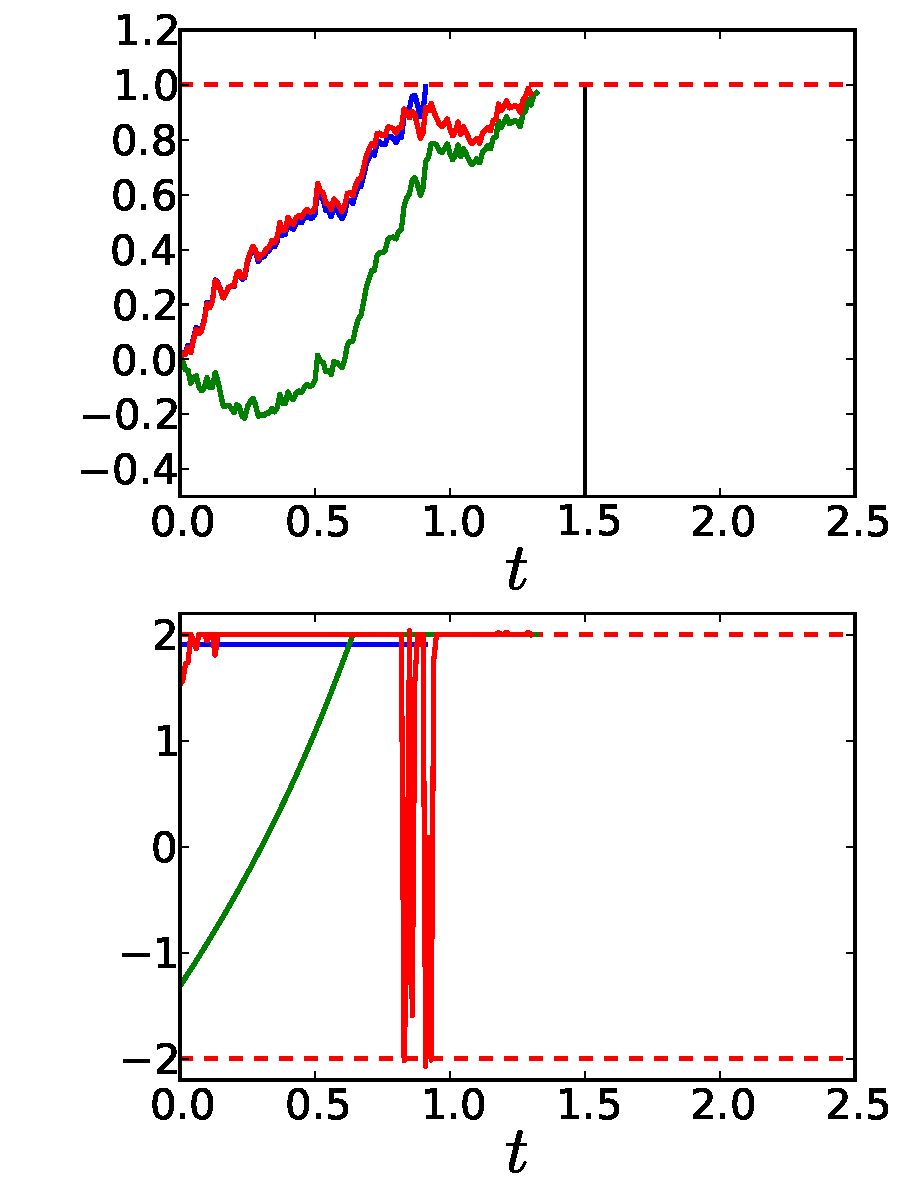
\includegraphics[width=0.3\textwidth]
{Figs/ControlSimulator/SubTLowNoise_Traj4.pdf}
}
\subfloat 
{
\label{fig:controlled_traj_ex2}
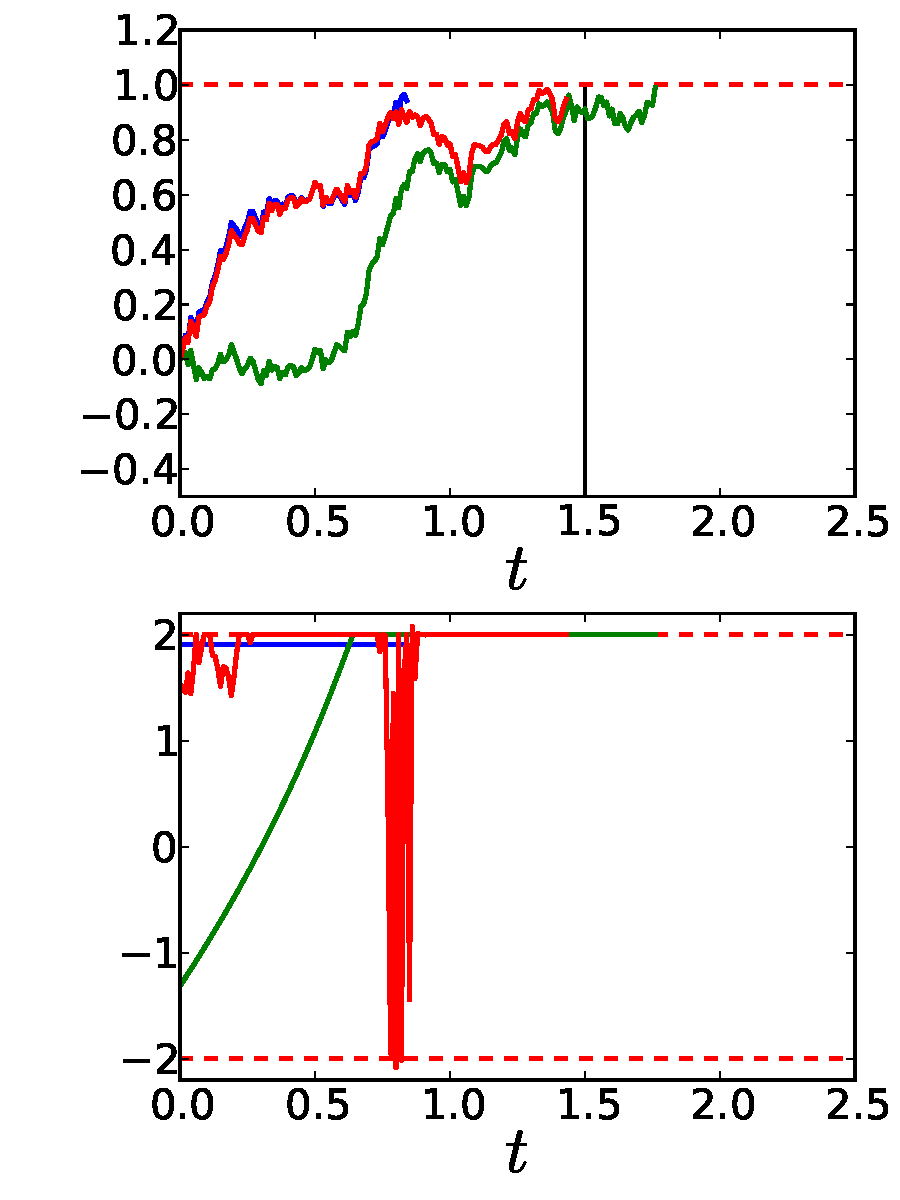
\includegraphics[width=0.3\textwidth] 
{Figs/ControlSimulator/SubTLowNoise_Traj6.pdf}
}
\subfloat
{
\label{fig:controlled_traj_ex3}
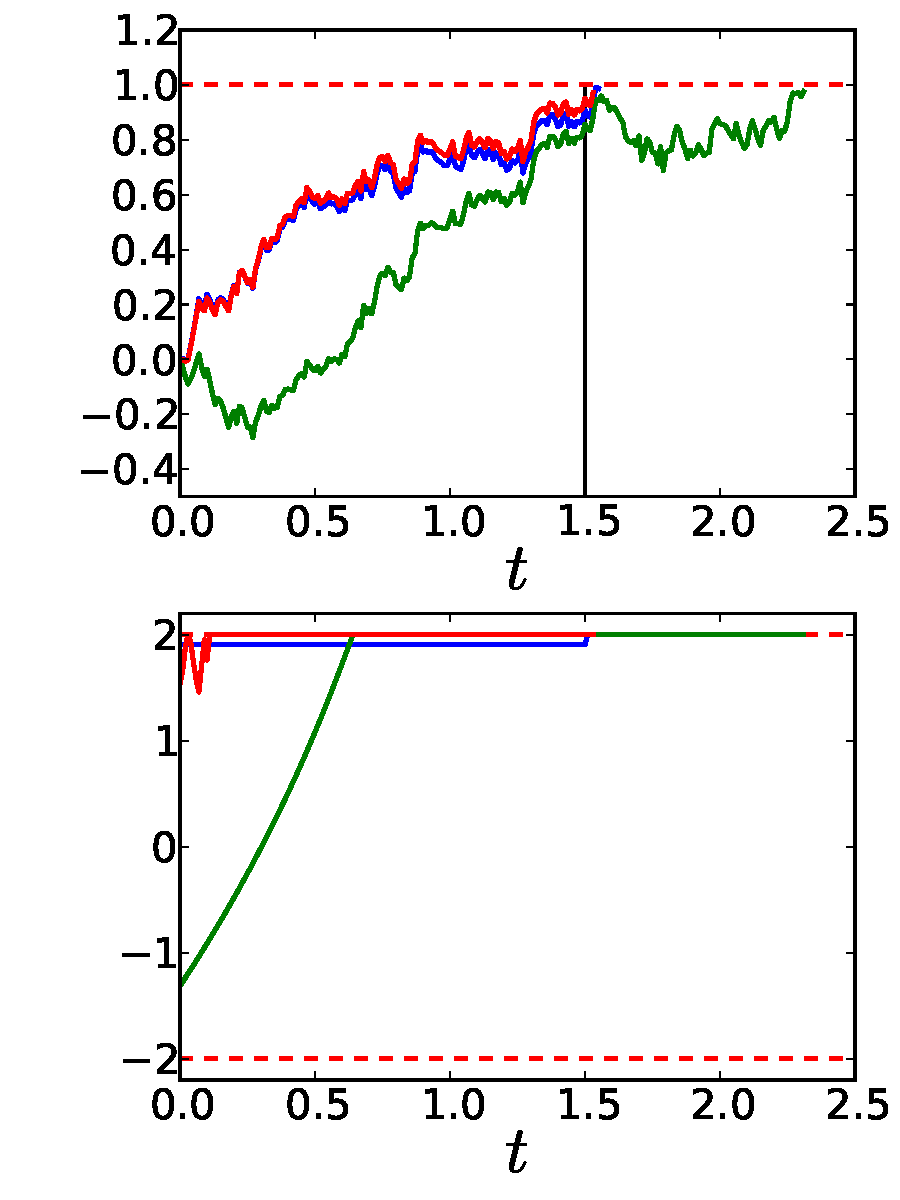
\includegraphics[width=0.3\textwidth]
{Figs/ControlSimulator/SubTLowNoise_Traj7.pdf}
}
\caption[]{Example Trajectories - Low Noise}
\end{center}
\end{figure}  
}

\only<2> {
\begin{figure}[h]
\begin{center} 
  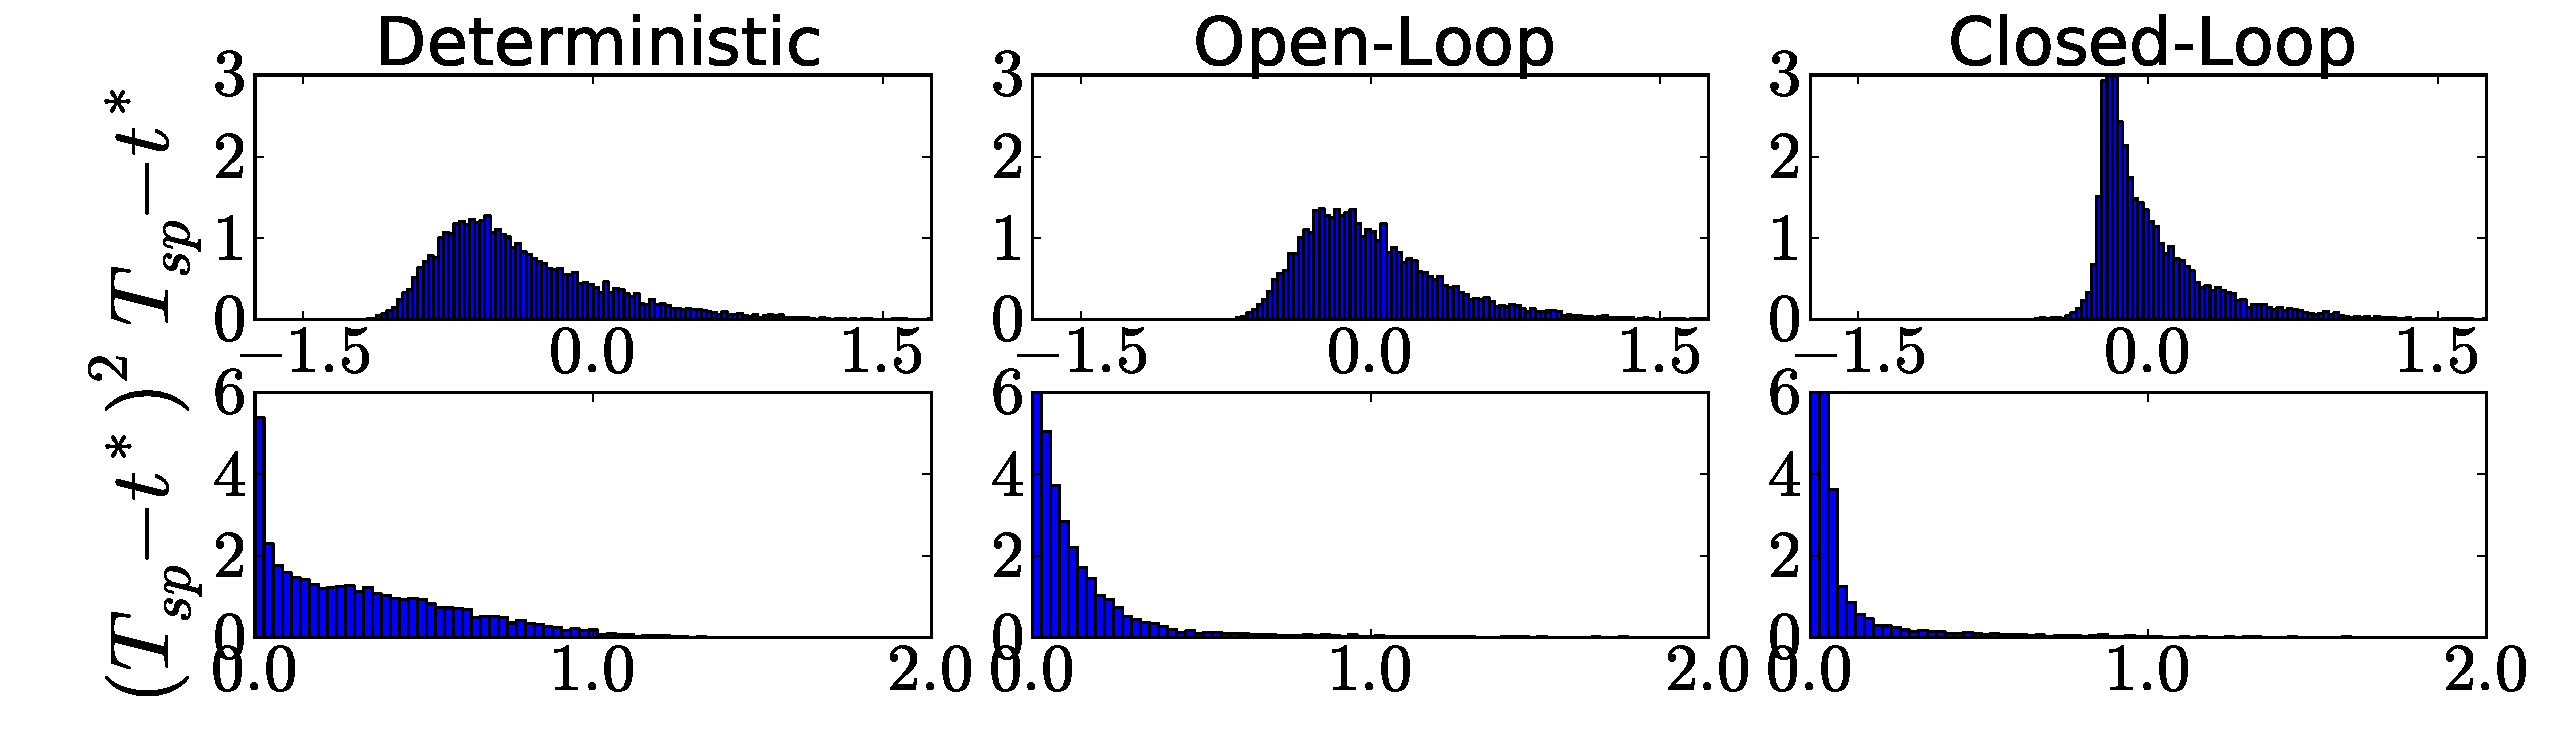
\includegraphics[width=.99\textwidth]
  {Figs/ControlSimulator/Regimes_subt_ln_errors_hist.pdf}
  \caption{Performance Histograms - Low Noise}
\end{center}
\end{figure}
}
\end{frame}


\begin{frame}
% \frametitle{A more fair comparison}
\frametitle{Simulation Comparison}
\only<1>{

\begin{figure}[h]
\begin{center}
\subfloat
{
\label{fig:controlled_traj_ex1}
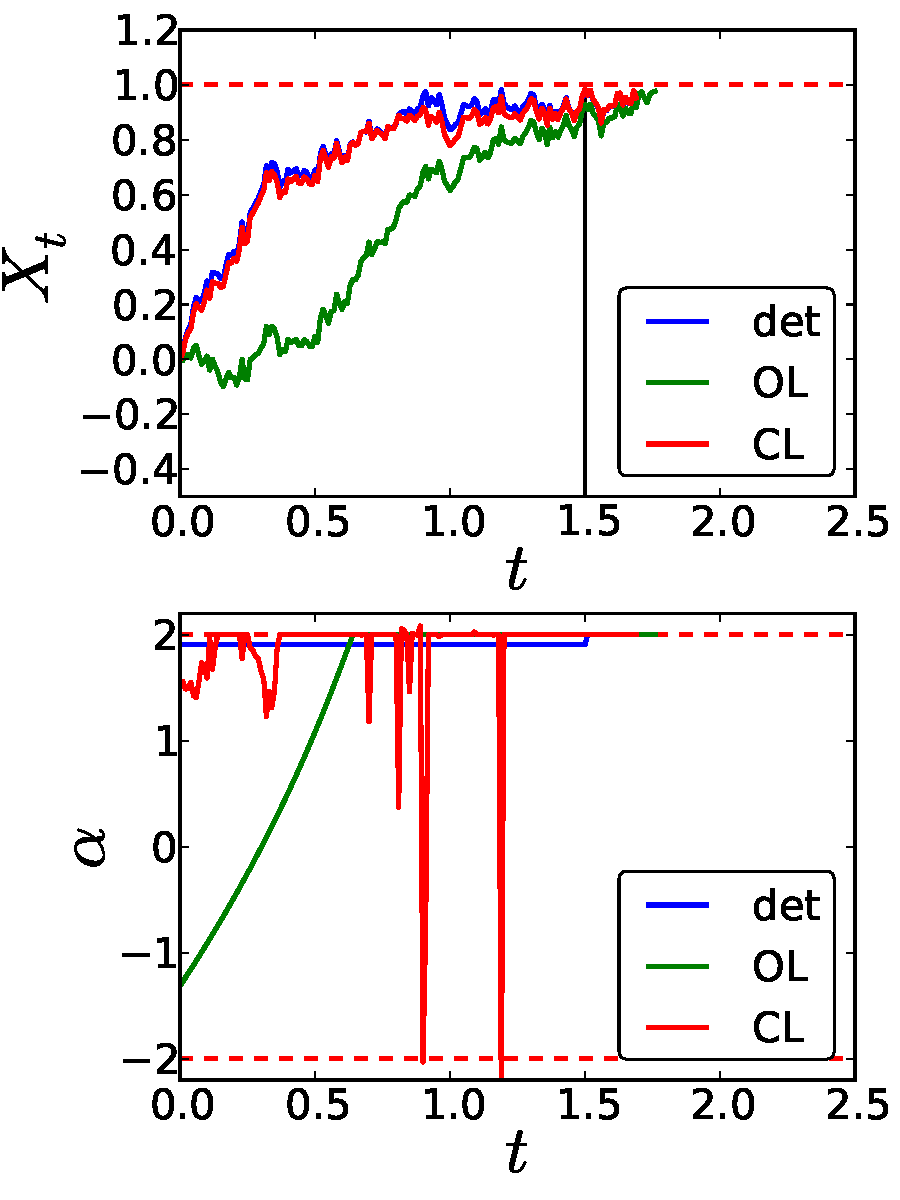
\includegraphics[width=0.3\textwidth]
{Figs/ControlSimulator/SubTHighNoise_Traj5.pdf}
}
\subfloat 
{
\label{fig:controlled_traj_ex2}
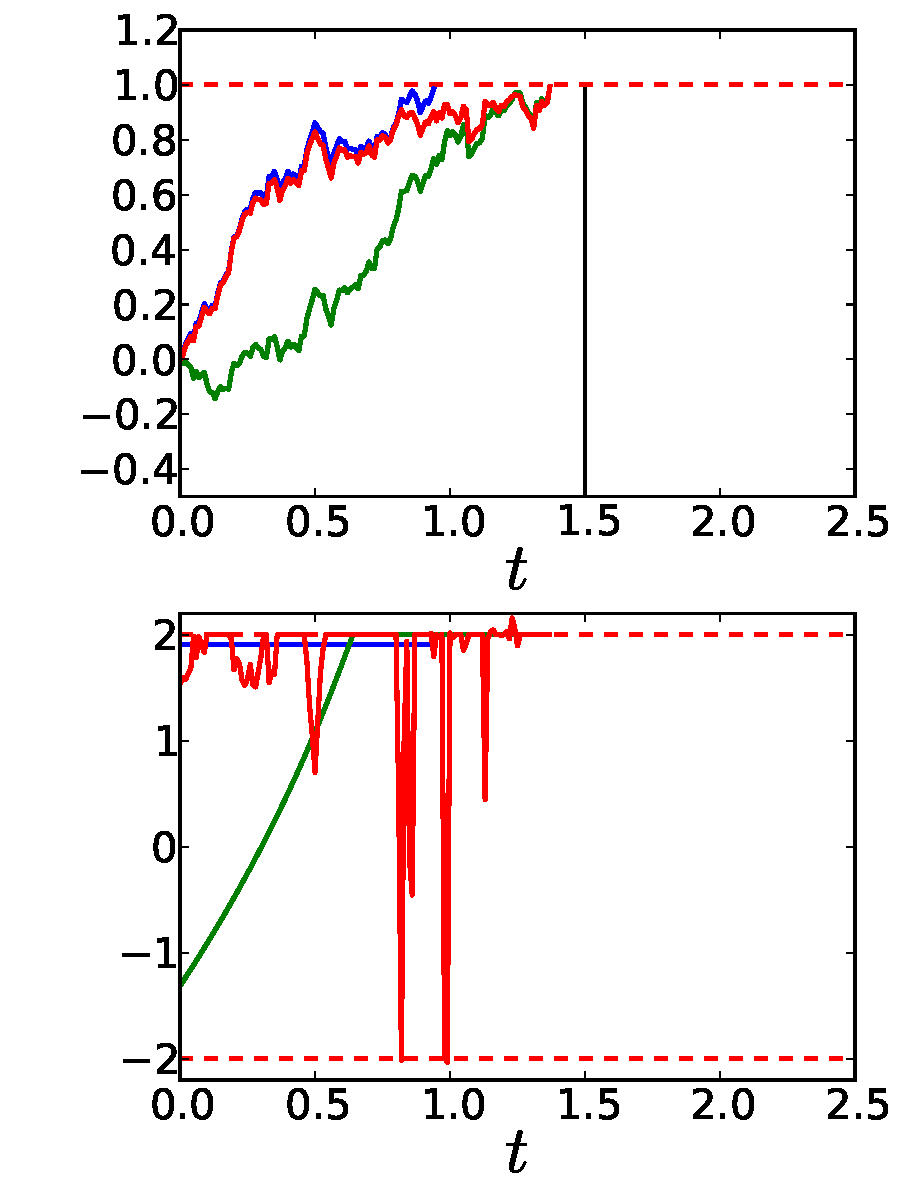
\includegraphics[width=0.3\textwidth] 
{Figs/ControlSimulator/SubTHighNoise_Traj3.pdf}
}
\subfloat
{
\label{fig:controlled_traj_ex3}
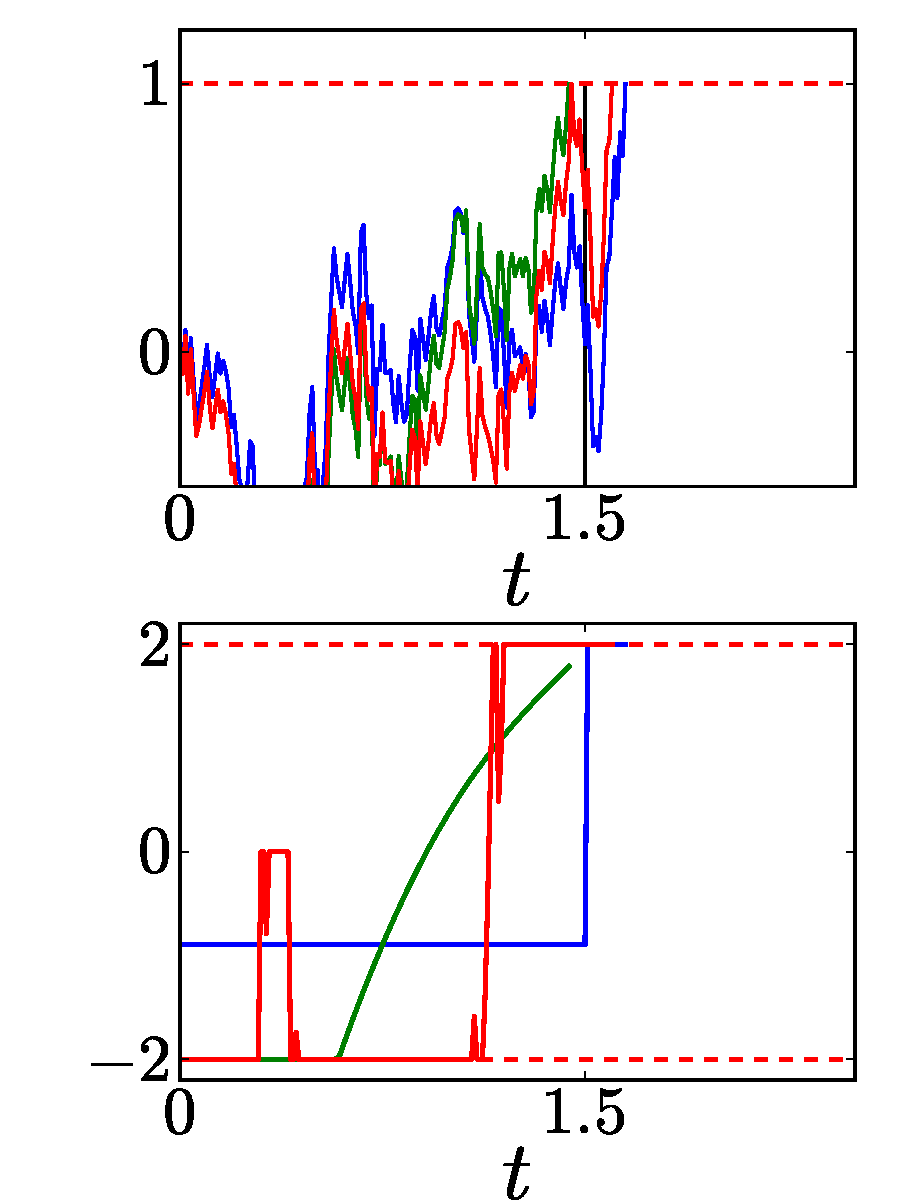
\includegraphics[width=0.3\textwidth]
{Figs/ControlSimulator/SubTHighNoise_Traj7.pdf}
}
\caption[]{Example Trajectories - High Noise}
\end{center}
\end{figure}  
}

\only<2> {
\begin{figure}[h]
\begin{center}
  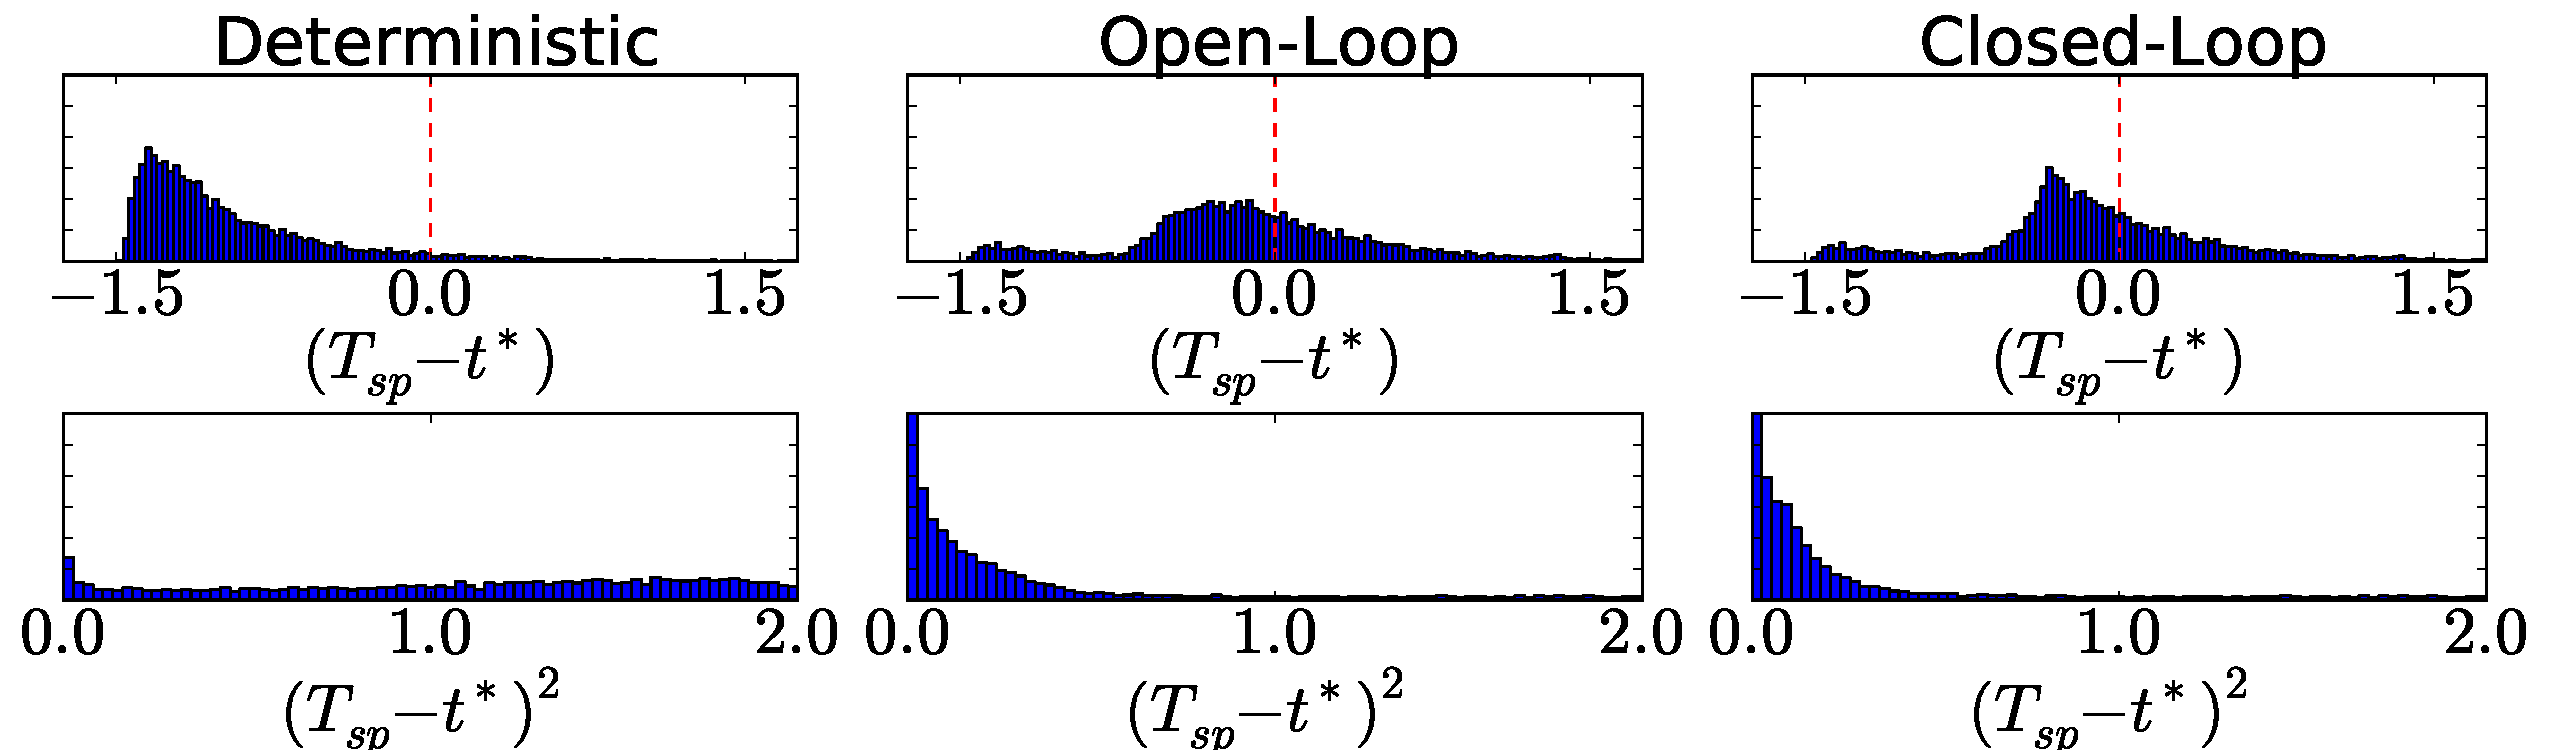
\includegraphics[width=.99\textwidth]
  {Figs/ControlSimulator/Regimes_subt_HN_errors_hist.pdf}
  \caption{Performance Histograms - High Noise}
\end{center}
\end{figure} 
}
\end{frame}


\begin{frame}
\frametitle{Our Goal}
Return to 
Target Train:

\begin{figure}
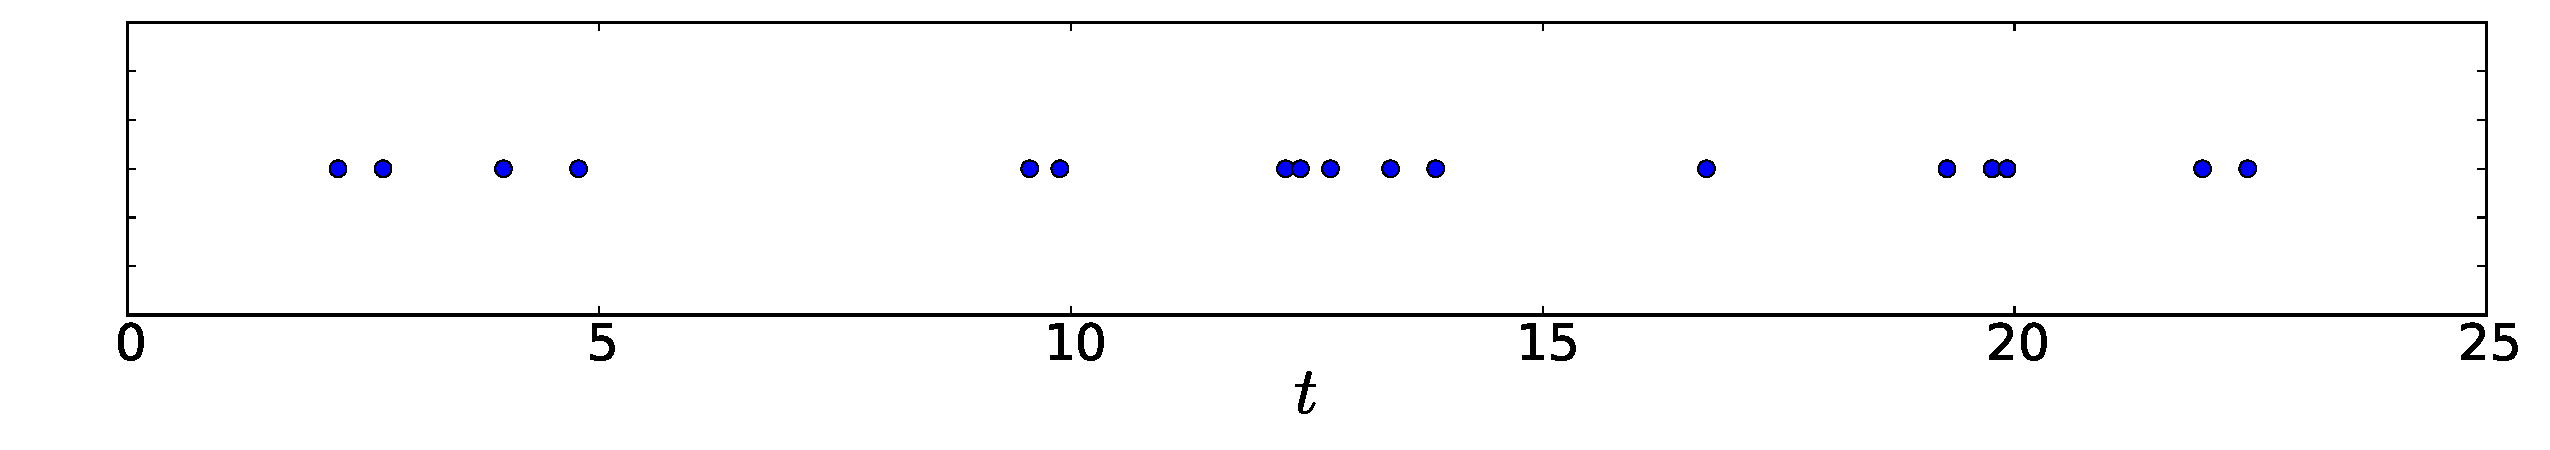
\includegraphics[width=0.9\textwidth]
{Figs/TrainController/target_train_Ahmadian.pdf}
\end{figure}

\vskip 3pt

Use:
\begin{table}
\begin{tabular}{|l|c|}
\hline
$\m$  & $2.0$ \\
\hline
$\b $ & .3 (Low Noise)\\ 
\hline
$\tc$ & .5 \\
\hline
$\m \cdot \tc $ & $1 = \xth$ \\
\hline
\end{tabular}
\end{table}


\end{frame}

\begin{frame}
\begin{figure}[htp]     
\begin{center}  
  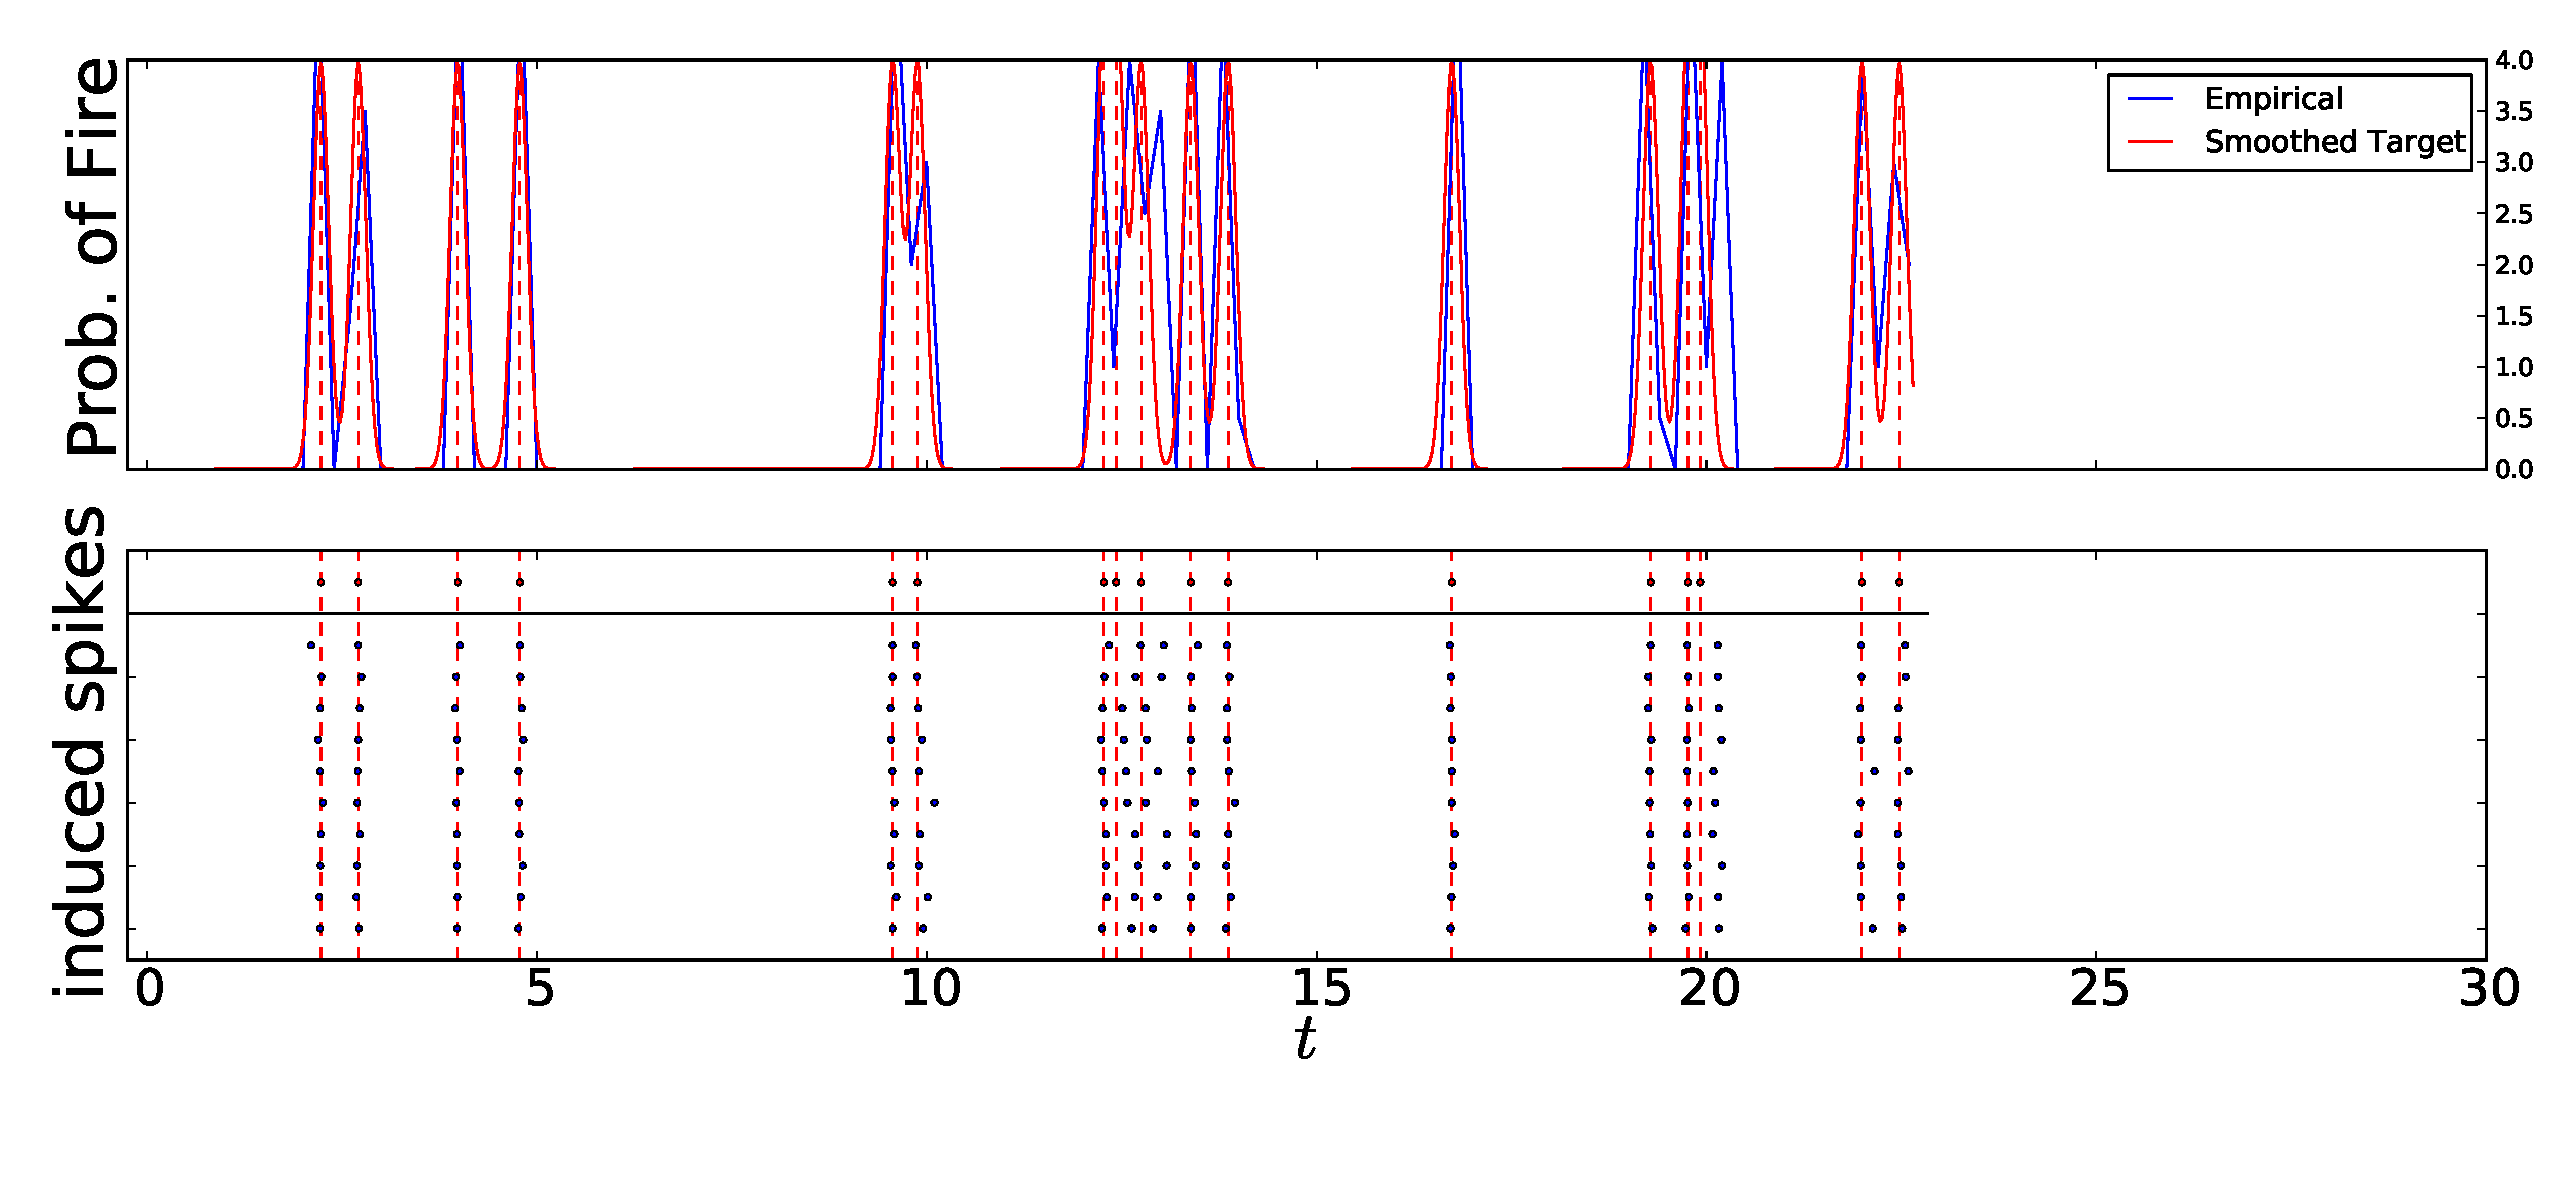
\includegraphics[width=.99\textwidth]{Figs/TrainController/CRITLN_Ahmadian_cl_trains_sim_10.pdf}
  \caption[ ]{Closed-loop (Dynamic Programing) Performance}
  \label{fig:targettrain_cl_critlownoise}  
\end{center}
\end{figure}   
\end{frame}
\begin{frame}
\begin{figure}[htp]     
\begin{center}  
  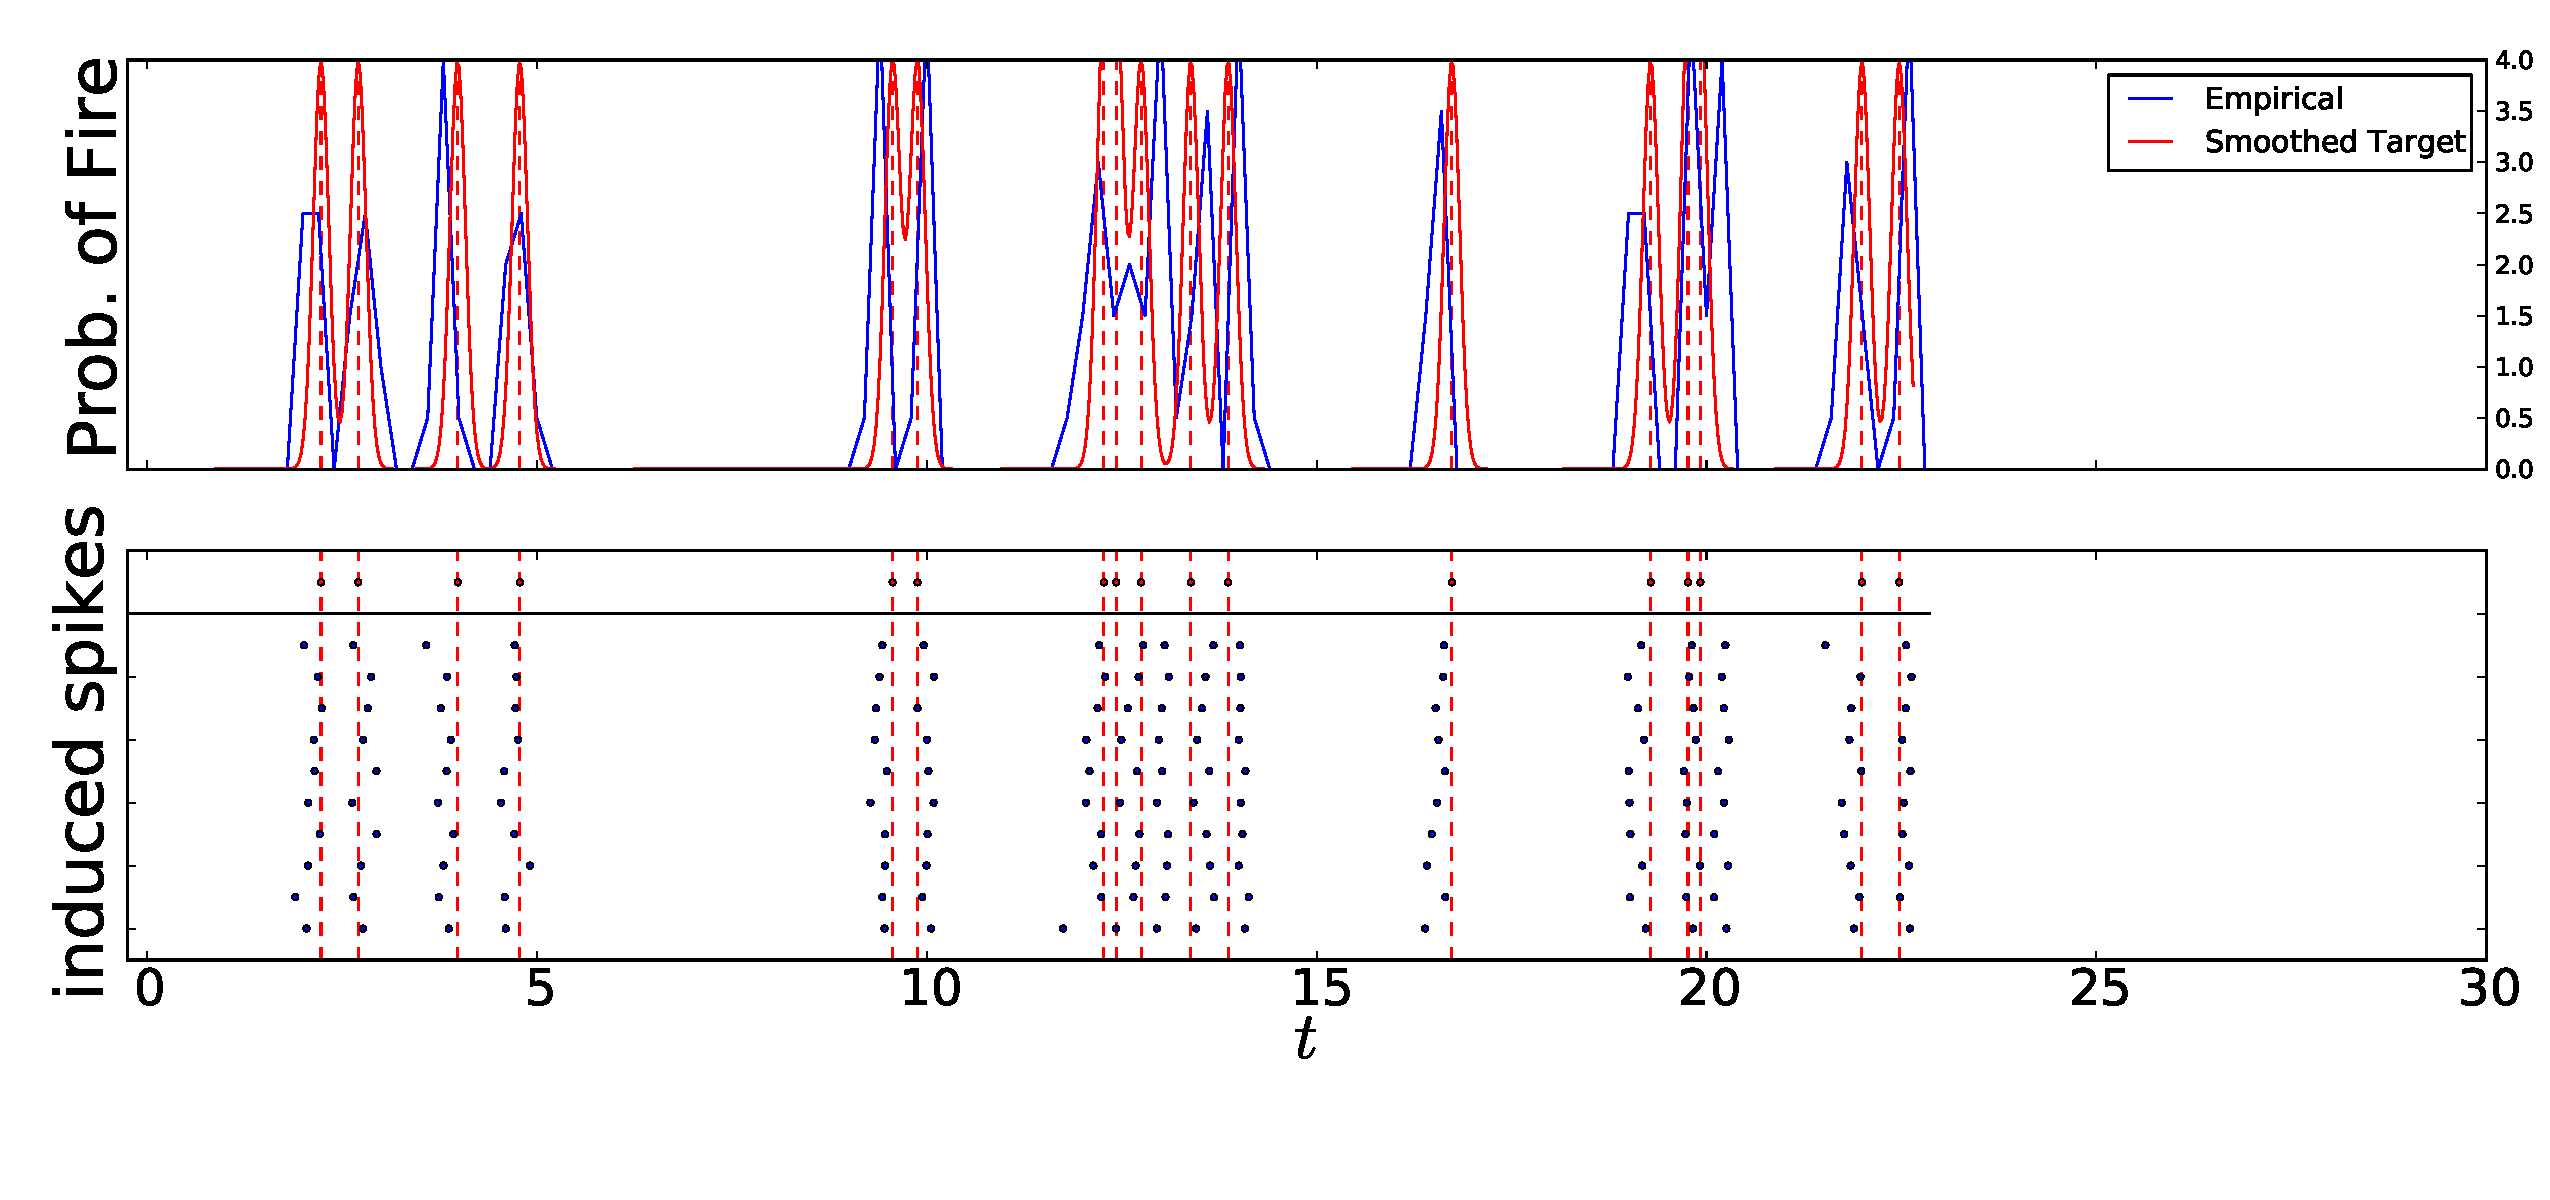
\includegraphics[width=.99\textwidth]
  {Figs/TrainController/CRITLN_Ahmadian_ol_trains_sim_10.pdf}
  \caption[ ]{Open-loop (Maximum Principle) Performance}
\end{center}
\end{figure}  
\end{frame}

\section*{Summary}

\begin{frame}
\frametitle<presentation>{Summary}
\begin{block}{Targeting Neural Trains}
  \begin{itemize}
    \item Eliciting a given Spike Train from a Neuron is reduced to controling a
    Sequence of First-Passage Times for a Ornstein-Uhlenbeck Process \pause
    \item The sequence is controlled independently for each hitting time \pause
	\item Given voltage observations - we use dynamic programing \pause
	\item With only spike observations - we use a maximum principle for the
	transition density \pause
	\item Online implementation should be difficult (the approach is
	computationaly heavy) 
  \end{itemize}
\end{block}

% \vskip0pt plus.5fill

% \begin{block}{To be addressed:}
%   \begin{itemize}
%     \item Where to apply this?
%   \end{itemize}
% \end{block}

\end{frame}

\end{document}
